\documentclass[xcolor={dvipsnames}]{beamer}
%\documentclass[handout,xcolor={dvipsnames}]{beamer}
\usepackage{lmodern}
% MD: we can mess with this ...
%\usetheme{Berlin}
%\usetheme{Goettingen}
% ... or use the IU style we've defined before:
%\usepackage{iucl}
%\usepackage[dvipsnames]{xcolor}
\usepackage{array}
\usepackage{graphicx}
\usepackage{tikz-dependency}
\usepackage{natbib}
\usepackage{url}
\usepackage{gb4e}
\usepackage{tikz-qtree}
%\usepackage{caption}

\makeatletter

\newcommand*{\@rowstyle}{}

\newcommand*{\rowstyle}[1]{% sets the style of the next row
  \gdef\@rowstyle{#1}%
  \@rowstyle\ignorespaces%
}

\newcolumntype{=}{% resets the row style
  >{\gdef\@rowstyle{}}%
}

\newcolumntype{+}{% adds the current row style to the next column
  >{\@rowstyle}%
}

\makeatother

\newcolumntype{C}[1]{>{\centering\arraybackslash}p{#1}}

\newcommand{\feat}[1]{\textsc{#1}}
\newcommand{\param}[1]{\texttt{#1}}
\newcommand{\md}[1]{\marginpar{\scriptsize MD: #1}}
\newcommand{\lk}[1]{\marginpar{\scriptsize LK: #1}}
% for removing all marginpars ==> good for final submission! %%nice trick!
\renewcommand{\marginpar}[1]{}

%%%
\setbeamertemplate{itemize/enumerate body begin}{\small}
\setbeamertemplate{itemize/enumerate subbody begin}{\small}
\setbeamertemplate{itemize/enumerate subsubbody begin}{\small}
%%%



% workaround for weird \newblock problem
% http://www.isi.edu/~johnh/SOFTWARE/uclathes.html
\def\newblock{\hskip .11em plus .33em minus .07em}

% MD: changing tables so we don't need these
\usepackage{multirow}
% \usepackage{rotating}
% \usepackage{booktabs}

\title{Semantic Analysis of \\ Image-Based Learner Sentences}
\author[Levi King]{Levi King\\
Indiana University  }
\date{August 6, 2021}


\setbeamerfont{page number in head/foot}{size=\footnotesize}
\setbeamertemplate{footline}[frame number]
\begin{document}

\maketitle
%\section{Background}
\begin{frame}
\frametitle{Background \& Motivation}
%\vspace{-4ex}
\begin{itemize}
\pause
\item Most intelligent computer-assisted language learning (ICALL) applications (\textit{Rosetta Stone}, \textit{Duo Lingo}, etc.) rely on outdated, ineffective methods:
\begin{itemize}
\pause
\item rote memorization \& grammatical error detection; menu-based vs. free input;
\pause
\item \textit{``engineering first''}: no second language acquisition (SLA), pedagogy, psychometrics
\end{itemize}
\pause
\item  SLA research $\rightarrow$ communicative \& task based learning
\end{itemize}

\small
\pause
\textit{How can we bridge this gap?}

\begin{itemize}
\pause
\item My vision: \pause open source app; transparent; pipeline of existing tools;
\pause
\item teachers create new games/stories by adding visual prompts and crowdsourcing native speaker (NS) responses;
\pause
\item use NS model to evaluate non-native speaker (NNS) responses
\end{itemize}
\end{frame}


%\section{Background}
%\begin{frame}
%\frametitle{Background \& Motivation}
%\small
%How can we provide L2 learners interactive, meaningful practice?
%\begin{itemize}
%\item Communicative \& task based learning vs. rote memorization and grammatical error detection \citep[e.g.,][]{leacock:ea:14}.
%%\item Second language acquisition (SLA) research has shown this to be largely ineffective; real communication and task-based learning are more effective \citep[cf.][]{CelceMurcia:2002:GrammarThroughContext, LarsenFreeman:1991:TeachingGrammar}.
%\end{itemize}
%
%\medskip
%Can we evaluate non-native speaker (NNS) data with models from crowdsourced native speaker (NS) data?
%
%\medskip
%\begin{itemize}
%\item My dissertation aims to show that we can combine NLP tools and SLA to create tutoring applications that are reliable, pedagogically sound and sufficiently transparent to allow for meaningful feedback.
%\end{itemize}
%\end{frame}

\begin{frame}
\frametitle{Research Questions}
%\vspace{-4ex}
\small
\pause
%My work here relies on images to constrain the range of responses to a predictable and manageable set of meanings. For semantic analysis of these image-based sentences to proceed, one must have a notion of what are necessary and sufficient parts of the image for NNSs to describe. To annotate this by hand is costly, whereas collecting comparable responses from NSs is relatively easy. This leads directly to the first two research questions:
\begin{itemize}
\pause
\vspace{1em}
\item[RQ1.]{Are the picture description task (PDT) responses of L2 English learners sufficiently similar to those of NSs to allow automatic evaluation based on a collection of NS responses?}
%In other words, do learners demonstrate significant overlap with native-like usage in a picture description task (PDT) setting?} %What differences exist and what NLP tools are needed to account for them?
\vspace{1em}
\pause
\item[RQ2.]{For PDT responses, what are appropriate representations for the purpose of providing meaning-oriented feedback or evaluation?}
% In other words, which linguistic components are crucial and which are superfluous?}
%As mentioned above, one goal of this project is to show that content-based evaluation of learner sentences is possible without the expense of developing major new tools or language resources; in this vein, the third research question is: 

%With the goal of automatic response scoring, these desired components of linguistic analysis and representation can guide decisions regarding the forming of an appropriate NLP pipeline. The next three research questions primarily address the relevant NLP concerns:
\pause
\vspace{1em}
\item[RQ3.]{What kinds of NLP tools are appropriate here?}
%As discussed later, this work attempts to take statistical methods traditionally used to analyze the frequencies of individual words in sentences and apply those methods to the frequencies of syntactic dependencies in sentences, as one means of deriving semantic information from syntactic tools. Thus, the fourth research question is:

\pause
\vspace{1em}
\item[RQ4.]{How do ``bag-of-words'' and ``bag-of-dependencies'' approaches compare in terms of performance?}
%Given that the system has thus far relied primarily on a parser, lemmatizer and spelling correction module, without the inclusion of semantic tools, the fifth research question is: %and given NLP trends that focus on surface forms over deeper processing...
\pause
\vspace{1em}
\item[RQ5.]{Can the accuracy of the system be improved with information from semantic tools (e.g., BERT)?}
%%Are increases in performance valuable enough to offset the computational costs? In other words, how deep should the processing be in order to achieve our goal of providing a meaning-based ICALL component that is lightweight and practical?} %%%**How deep should the processing be?

%The processing of unannotated responses is a primary goal of this work, but in order to evaluate the output of my system, manually annotated responses are necessary. In keeping with the motivations of this dissertation, the annotation should capture response accuracy and appropriateness. My sixth and final research question focuses on these concerns:
\pause
\vspace{1em}
\item[RQ6.]{What is the annotation scheme for this task and can the system perform within the range of human performance?}
\end{itemize}
\end{frame}

%\begin{frame}
%\frametitle{Accomplishments}
%%\vspace{-4ex}
%\small
%\pause
%Developed basic mechanism:
%\begin{itemize}
%\pause
%\item dependency parsing \& lemmatization \pause $\rightarrow$ dependency-level tf-idf \pause $\rightarrow$ vectorize NS \& NNS responses \pause $\rightarrow$ cosine $=$ response score;
%\pause
%\item Optimized system settings:
%\pause
%\begin{itemize}
%\item item type: intransitive, transitive, ditransitive actions
%\pause
%\item item complexity (type-to-token ratios, avg NS response length)
%\end{itemize}
%\end{itemize}
%\pause
%But first -- \textit{all of this required appropriate data!}
%\begin{itemize}
%\pause
%\item evaluating my system, finding trends, optimizing;
%\pause
%\item created task, collected data from 499 participants; $\approxeq$14,000 responses, NS $+$ NNS;
%\pause
%\item developed \& implemented meaning-focused annotation scheme;
%\pause
%\item established feature weights for scoring \& ranking NNS (benchmark);
%\end{itemize}
%\end{frame}
%
\begin{frame}
\frametitle{System}

%\vspace{-1.2em}
\textbf{Step 1: Dependency parse:}

\begin{figure}[htb!]
\begin{center}
    \begin{dependency}[arc edge,text only label,label style={above}]
    \begin{deptext}[column sep=.5em]
      \textit{vroot} \& The \& boy \& is \&[1em] eating \& pizza \\
    \end{deptext}
    \depedge[arc angle=78]{1}{5}{root}
    \depedge[arc angle=35]{3}{2}{det}
    \depedge[arc angle=65,edge style={double}]{5}{3}{nsubj}
    \depedge[arc angle=20]{5}{4}{aux}
    \depedge[edge style={double}]{5}{6}{dobj}
%    \depedge[arc angle=35,edge style={dotted}]{7}{6}{det}
%    \depedge[edge style={dotted}]{3}{2}{det}
  \end{dependency}
\end{center}
%\caption{The dependency parse}
\label{fig:prep-dependency}
\end{figure}

\begin{columns}
\pause
\column{0.2\textwidth}

    \column{0.4\textwidth}
%        \centering
\begin{table}
\begin{tabular}{l}
\textbf{Get dependencies:} \\
% & \\
root(eating, \textit{vroot}) \\
det(the, boy) \\
nsubj(boy, eating) \\
aux(is, eating) \\
dobj(pizza, eating) \\
\end{tabular}
\end{table}

%\column{0.3\textwidth}
%        \centering
%\begin{table}
%\begin{tabular}{l}
%Step 2: Lemmatize:
%\\
%\\
%$\rightarrow$ \\
%\\
%\end{tabular}
%\end{table}

\pause
\column{0.4\textwidth}
%        \centering
\begin{table}
\begin{tabular}{cl}
\multicolumn{2}{c}{\textbf{Step 2: Lemmatize:}} \\
% & \\
$\rightarrow$ & root(\textbf{eat}, \textit{vroot}) \\
$\rightarrow$ & det(the, boy) \\
$\rightarrow$ & nsubj(boy, \textbf{eat}) \\
$\rightarrow$ & aux(\textbf{be}, \textbf{eat}) \\
$\rightarrow$ & dobj(pizza, \textbf{eat}) \\
\end{tabular}
\end{table}

\column{0.2\textwidth}

\end{columns}

\end{frame}

\begin{frame}
\frametitle{System}
%\vspace{-2em}
\small
\textbf{Step 3: tf-idf} (term frequency-inverse document frequency) \\
\vspace{.5em}
\pause
NS model: [He is eating pizza. The boy is eating pizza.] \\ 
\vspace{.5em}
\pause
NNS 1: He is eating food. \hspace{1.4em} \pause NNS 2: He is eating pizza. \\

\pause
\vspace{-.6em}
\footnotesize
\begin{table}[htb!]
%\vspace{.3em}
\begin{center}
\begin{tabular}{|c||c|c||c|c||c|c|}
\hline
 & \multicolumn{2}{c||}{NS model} & \multicolumn{2}{c||}{NNS 1} & \multicolumn{2}{c|}{NNS 2} \\
\cline{2-7}
NS $\cup$ NNSs & tf & tf-idf & tf & tf-idf & tf & tf-idf \\
\hline
aux(be,eat) & 2 & .04 & 1  &  .02 &  1 & .02 \\ 
\hline
det(the,boy) & 1 & .04 &  -  & 0 & - & 0 \\
\hline
dobj(food,eat) & - & 0 & 1   & .06 & - & 0 \\
\hline
dobj(pizza,eat) & 2 & .16 & -   & 0 & 1 & .08 \\
\hline
nsubj(boy,eat) & 1 & .08 & -  & 0 & - & 0 \\
\hline
nsubj(he,eat) & 1 & .04 & 1   & .02 & 1 & .02 \\
\hline
root(eat,vroot) & 2 & .02 & 1   & .01 & 1 & .01 \\ %.02
\hline
\end{tabular}
\end{center}
\end{table}

\vspace{.5em}

\small
Response scores: cosine(NS model tf-idf, NNS tf-idf) \\
\vspace{.5em}

\pause
NNS 1: 0.139 \hspace{.6em} \pause NNS 2: 0.886 \pause \hspace{.6em} $\rightarrow$ \hspace{.6em} \textit{NNS 2 is closest to the model.} \\

\end{frame}

\begin{frame}
\frametitle{Data collection}
\medskip

PDT with very simple images only:

\begin{figure}[htb!]
\begin{center}
\begin{tabular}{|c|c|}
\hline
{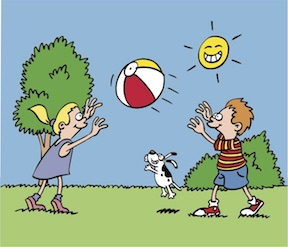
\includegraphics[width=0.38\columnwidth]{figures/throw-original.jpg}} & {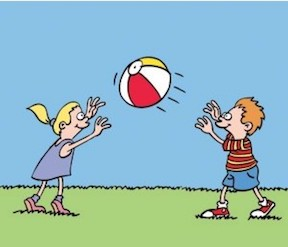
\includegraphics[width=0.38\columnwidth]{figures/I21cropped.jpg}} \\
\hline
Original image & Simplified PDT image \\
\hline
\end{tabular}
%\caption{\label{fig:image-prep} All non-essential details were removed from the PDT images in order to focus participants' attention on the main action.}
\end{center}
\end{figure}

Intended to focus participants' attention on the main action
\end{frame}

\begin{frame}
\frametitle{Data collection}

Two PDT prompt versions:
%\begin{itemize}
%\item \textbf{Targeted} 
%\begin{itemize}
%\item \textit{What is the $<$subject$>$ doing?} 
%\end{itemize}
%\item \textbf{Untargeted} 
%\begin{itemize}
%\item \textit{What is happening?} 
%\end{itemize}
%\end{itemize}
\begin{figure}[htb!]
\begin{center}
%\begin{tabular}{|c|c|}
\begin{tabular}{|C{50mm}|C{50mm}|}
\hline
\textbf{Targeted} & \textbf{Untargeted} \\
\hline
{
\includegraphics[trim=0 50 0 50,clip,width=0.33\columnwidth]{figures/I10.jpg}} & {
\includegraphics[trim=0 50 0 50,clip,width=0.33\columnwidth]{figures/I10.jpg}} \\
\hline
\textit{What is \textbf{the baby} doing?} & \textit{What is happening?} \\
\hline
\end{tabular}
%\caption{\label{fig:image-prep} All non-essential details were removed from the PDT images in order to focus participants' attention on the main action.}
\end{center}
\end{figure}

Intended for exploring the specificity needed for my approach

\end{frame}

\begin{frame}
\frametitle{Data collection}

3 verb types:

\begin{table}[width=.8\columnwidth]\small
\begin{center}
\begin{tabular}{|C{33.5mm}|C{34mm}|C{33.5mm}|}
\hline
10 \textbf{intransitive} items & 10 \textbf{transitive} items & 10 \textbf{ditransitive} items \\
\hline
{
\includegraphics[width=0.2\columnwidth]{figures/I20.jpg}} & {
\includegraphics[width=0.2\columnwidth]{figures/I02.jpg}} &
{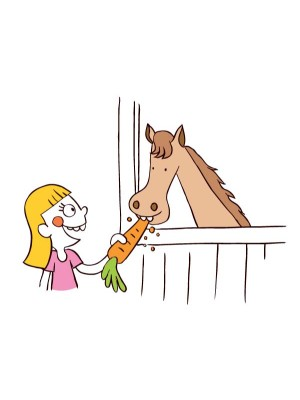
\includegraphics[trim=21 90 65 110,clip,width=0.25\columnwidth]{figures/I17.jpg}} \\
\hline
What is the girl doing? & What is the boy doing? & What is the girl doing? \\
\hline
\end{tabular}
\end{center}
\end{table}

Intended for exploring whether my approach can generalize to a range of sentence types
\end{frame}


\begin{frame}{Data collection}

\vspace{1em}
The pilot study \textit{rake} problem; 100\% of NS used the verb \textit{rake}:


\begin{figure}[htb!]
\begin{center}
\bgroup
\def\arraystretch{1.25}
\begin{tabular}{|C{35mm}|C{65mm}|}
\hline
\multirow{5}{*}{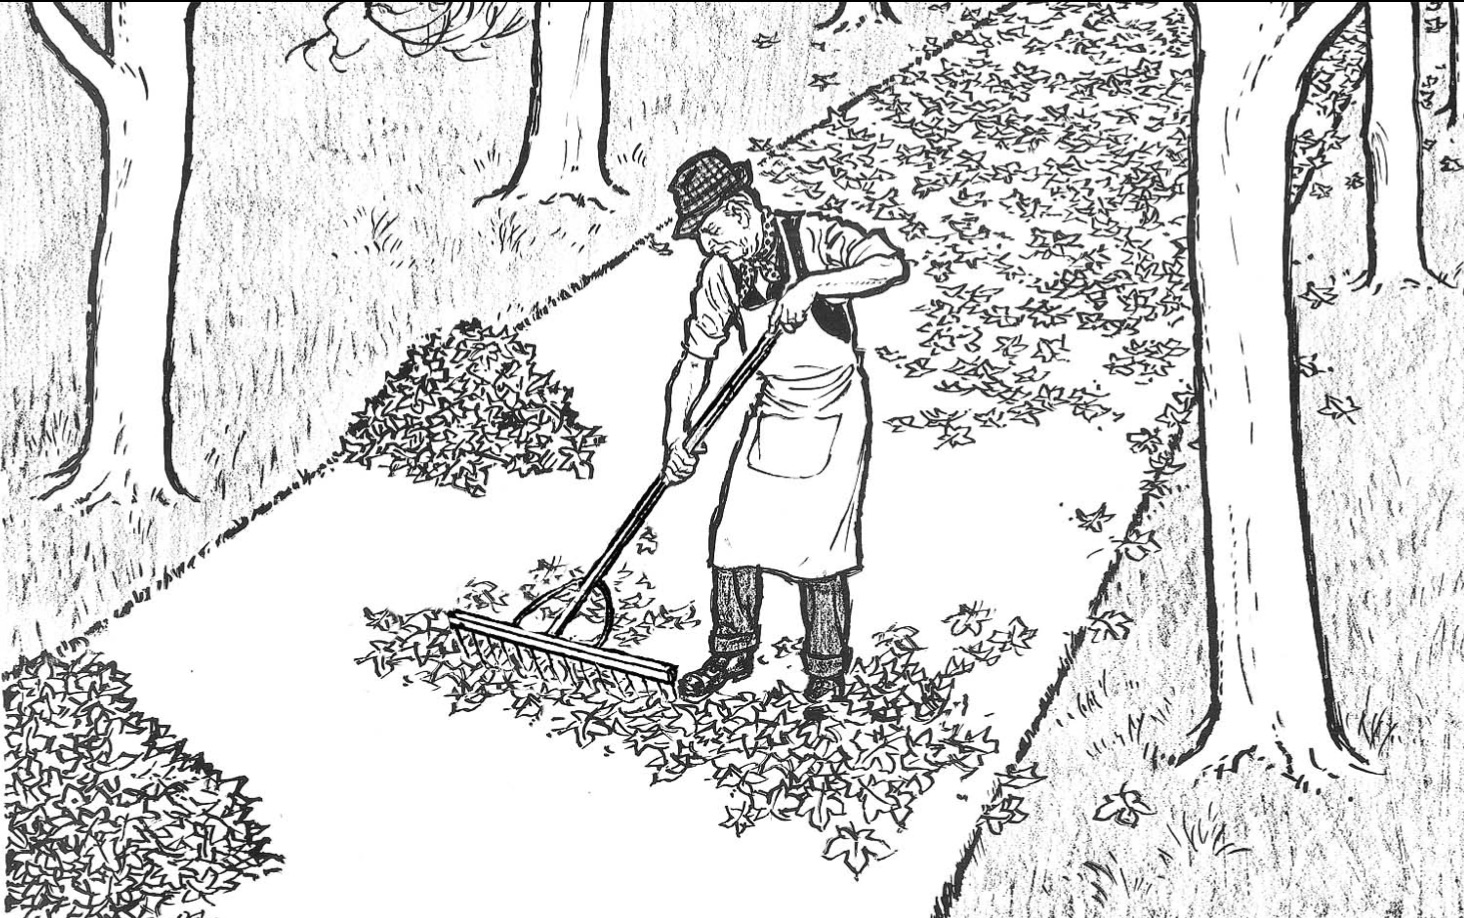
\includegraphics[trim=270 90 300 100,clip,width=0.34\columnwidth]{figures/rake.jpg}} &
\textbf{NNS Responses} \\
\cline{2-2}
& The gardener is \textit{cleaning} the street. \\
\cline{2-2}
& a man \textit{removing} the tree leafs. \\
\cline{2-2}
& The man is \textit{sweeping} the floor. \\
\cline{2-2}
& A man is \textit{gathering} lots of leafs. \\
\hline
\end{tabular}
\egroup
\end{center}
\label{fig:pilot-raking}
\end{figure}


\begin{itemize}
\item NNS responses without \textit{rake} are penalized;
\item I address this by asking NSs for two non-identical responses.
\end{itemize}
\end{frame}



\begin{frame}
\frametitle{Main study: Data collection}
\vspace{.5em}
499 participants, 13,533 responses:
\vspace{.5em}
\pause
\begin{itemize}
\pause
\item 141 NNSs (ELIP at IU), 4,290 responses;
\vspace{.5em}
\begin{itemize}
\pause
\item 125 Mandarin, 4 Korean, 3 Burmese, 2 Hindi; 1 each: Arabic, Indonesian, German, Gujarati, Spanish, Thai, Vietnamese;
\end{itemize}
\vspace{.5em}
\pause
\item 358 NSs, 9,243 responses:
\begin{itemize}
\pause
\vspace{.5em}
\item 329 \param{crowdsourced}, purchased via SurveyMonkey;
\pause
\begin{itemize}
\item 7,960 responses;
\end{itemize}
\pause
\vspace{.5em}
\item 29 \param{familiar}, unpaid colleagues;
\begin{itemize}
\item 1,283 responses;
\end{itemize}
\end{itemize}
\end{itemize}

%\vspace{-.2em}
%\begin{small}
%\begin{table}[htb!]
%\begin{center}
%\begin{tabular}{|l||r|r||r|}
%\hline
%& \multicolumn{3}{c|}{Response Counts} \\
%\hline
% Group & First & Second & Total \\
%\hline
%\hline
%NNS & 4290 & 0 & 4290 \\
%\hline
%\hline
%NS (all) & 4634 & 4609 & 9243 \\ %%LK: Yes, 0.949 is correct in both cases here
%\hline
%\multicolumn{1}{|r||}{\param{Familiar}} & 642 & 641 & 1283 \\ 
%\hline
%\multicolumn{1}{|r||}{\param{Crowdsrc}} & 3992 & 3968 & 7960 \\
%\hline
%\hline
%Total & 8924 & 4609 & \textbf{13,533} \\
%\hline
%\end{tabular}
%\end{center}
%\end{table}
%\end{small}

\end{frame}


\begin{frame}
\frametitle{Annotation features}
5 binary features:
\begin{itemize}
\pause
\vspace{.8em}
\item \feat{Core event}: \pause Does response capture main action?
\pause
\vspace{.8em}
\item \feat{Answerhood}: \pause Does response directly answer prompt?
\pause
\vspace{.8em}
\item \feat{Grammaticality}: \pause Is response free from grammar problems?
\pause
\vspace{.8em}
\item \feat{Interpretability}: \pause Does response evoke a clear mental image?
\pause
\vspace{.8em}
\item \feat{Verifiability}: \pause Is all response info supported by image?
\end{itemize}


\end{frame}

\begin{frame}
\frametitle{Annotation features}
\begin{table}[htb!]
\small
\textbf{C}ore event, \textbf{A}nswerhood, \textbf{G}rammaticality, \textbf{I}nterpretability, \textbf{V}erifiability \\

\vspace{.3em}
\begin{center}
%\begin{tabular}{|p{3.7cm}|c|c|c|c|c|}
\begin{tabular}{|l|c|c|c|c|c|}
\hline
\multicolumn{6}{|c|}{
\includegraphics[width=0.25\columnwidth]{figures/I02.jpg}} \\
\hline
\textit{What is the boy doing?} & C & A & G & I & V \\
\hline
\hline
He is eating food. & 0 & 1 & 1 & 1 & 1 \\
\hline
he eating pizza. & 1 & 1 & 0 & 1 & 1 \\
\hline
The boy is smiling pizza. & 0 & 1 & 0 & 0 & 0 \\
\hline
He may get fat eating. & 0 & 0 & 1 & 1 & 0 \\
\hline
\end{tabular}
%\caption{\label{tab:dev-transitive} \small Annotated for five features: Core event (\textit{C}), Answerhood (\textit{A}), Grammaticality (\textit{G}), Interpretability (\textit{I}) and Verifiability (\textit{V}).}
\end{center}
\end{table}
\vspace{.3em}

Inter-rater reliability (Cohen's kappa): 0.744 (\textbf{I}) -- 0.936 (\textbf{A}) \\

\end{frame}

\begin{frame}
\frametitle{Evaluating performance}

%\vspace{-2em}
Problem: My system scores are between 0 and 1, but annotation is 5 binary scores. How can I evaluate system performance? \\

\vspace{1em}
\pause
I need \textbf{benchmark rankings} for the NNS test set. \\

\pause
\vspace{1em}
Feature-level performance:
\begin{itemize}
\pause
\item \textbf{MAP} to see how system rankings predict \textbf{individual features};
\begin{itemize}
\pause
\item Compare with? Some \textit{holistic benchmark ranking} MAP;
\end{itemize}
\end{itemize}

\vspace{.3em}
\pause
Holistic performance (response quality):
\begin{itemize}
\pause
\item \textbf{Spearman} rank correlation: Compare system rankings with some \textit{holistic benchmark ranking};
%\begin{itemize}
%\item 
\end{itemize}
%\end{itemize}

\pause
\vspace{1em}
Solution: Determine feature weights and apply to annotations to obtain benchmark holistic scores and then rankings. \\
\end{frame}

\begin{frame}
\frametitle{Weighting features}

\vspace{1em}

Annotators performed a preference task for pairs of responses. \\

\vspace{.7em}

\pause
Feature weights were derived according to how frequently each feature is ``yes'' among preferred responses. \\

\vspace{1em}
\pause
\begin{table}[htb!]
\begin{center}
\begin{tabular}{|l|l|l|l|l|}
\hline
Core & Answr & Gramm & Interp & Verif \\
\hline
.365 & .093 & .055 & .224 & .263 \\
\hline
\end{tabular}
\end{center}
\end{table}

\vspace{1em}

\pause

Preferences are reliable:

\vspace{1em}

Agreement for two annotators on a sample of 300 pairs:

\vspace{1em}

\begin{table}[htb!]
\begin{center}
\begin{tabular}{|l|l|l|}
\hline
 Chance Agree & Observed Agree & Cohen's Kappa \\
\hline
0.621 & 0.883 (265/300) & 0.692 \\
\hline
\end{tabular}
%\caption{\label{tab:ABAgreement} Preference task agreement scores for two annotators on a sample of 300 response pairs; expected chance agreement, observed agreement and Cohen's Kappa.}
\end{center}
\end{table}

\end{frame}

\begin{frame}
\frametitle{Benchmark rankings}
\small
\begin{itemize}
\pause
\item Apply feature weights for weighted annotation scores (WAS);
\pause
\item Rank NNS test set by WAS for weighted annotation ranking (WAR);
\pause
\end{itemize}


\vspace{-1em}
\begin{footnotesize}
\begin{table}[htb!]
%Weight & 0.365 & 0.093 & 0.056 & 0.224 & 0.263 & 1.0 \\
\begin{center}
%\begin{tabular}{|l||r|r|r|r|r||r|r|}
\begin{tabular}{|p{2.7cm}||p{.7cm}|p{.7cm}|p{.7cm}|p{.7cm}|p{.7cm}|p{.7cm}|p{.6cm}|}
\hline
\textit{What is happening?} & C & A & G & I & V & WAS & WAR \\
\hline
\hline
The boy is eating pizza & 0.365 & 0.093 & 0.055 & 0.224 & 0.263 & 1.000 & 1 \\
\hline
Child is eating pizza & 0.365 & 0.093 & 0.000 & 0.224 & 0.263 & 0.945 & 2 \\
\hline
Tommy is eating pizza & 0.365 & 0.093 & 0.055 & 0.224 & 0.000 & 0.737 & 3 \\
\hline
The boy's eating his favorite food & 0.000 & 0.093 & 0.055 & 0.000 & 0.000 & 0.513 & 4 \\
\hline
Pizza is this boy's favorite food & 0.000 & 0.000 & 0.055 & 0.000 & 0.000 & 0.055 & 5 \\
\hline
\end{tabular}
%\caption{\label{tab:applied-weights} Example NNS responses (see Table~\ref{tab:dev-transitive}) with feature weights applied to the binary annotations, resulting in weighted annotation scores (\textit{WAS}) and a weighted annotation ranking (\textit{WAR}).}
\end{center}
\end{table}
\end{footnotesize}

%\pause
%\begin{itemize}
%\item Use WAR as benchmark;
%\begin{itemize}
%\item Features: Get MAP for WAR, compare against system MAP;
%\pause
%\item Holistic: Get Spearman for system ranking vs. WAR;
%\end{itemize}
%\end{itemize}

\end{frame}

\begin{frame}
\frametitle{SBERT for comparison}
I also use SBERT for comparing my system's performance.
\vspace{.3em}
\begin{itemize}
\pause
\item State-of-the-art sentence embedding for semantic textual similarity.
\vspace{.3em}
%\vspace{-1.2em}
\pause
\item Replaces dependency parser $+$ lemmatizer $+$ tf-idf cosine pipeline. 
\vspace{.3em}
\pause
\item Provides distance between NNS response and NS model.
%\vspace{.3em}
%\pause
%\item Operates directly on text, not dependencies.
%\begin{itemize}
%\vspace{.3em}
%\pause
%\item Term representation parameter (\param{ldh}, \param{xdh}, \param{xdx}) does not apply.
%\end{itemize}
\end{itemize}
\end{frame}


\begin{frame}
\frametitle{System configuration}
\small

\vspace{.8em}
%\pause
%Optimizing my system means searching for the settings that yield the best performance; i.e., system output best approximates benchmark (WAR). \\
Optimizing means finding the best system settings:

\begin{itemize}
\pause
\item \textbf{Transitivity}: \param{intransitive}, \param{transitive}, \param{ditransitive};
\pause
\item \textbf{Targeting}: \param{targeted}, \param{untargeted};
%\begin{itemize}
%\item \param{targeted}: \textit{What is $<$the subject$>$ doing?}
%\item \param{untargeted}: \textit{What is happening?}
%\end{itemize}
\pause
\item \textbf{Familiarity}: \param{familiar}, \param{crowdsourced}
\pause
\item \textbf{Primacy}:
\begin{itemize}
\item \param{primary}: NS model contains only 1st responses;
\item \param{mixed}: NS model: 1st \& 2nd responses (50-50);
\end{itemize}
\pause
\item \textbf{Term Representation}:
\begin{itemize}
\item \param{ldh}: label-dependent-head; i.e., labeled dependencies;
\item \param{xdh}: dependent-head; i.e., unlabeled dependencies;
\item \param{xdx}: dependent only; cf. \textit{bag of words};
\item Does not apply to SBERT (operates on plain text);
\end{itemize}
\end{itemize}

\vspace{.3em}
\pause
A \textbf{system configuration} combines one setting from each.

\end{frame}




%\begin{frame}
%\frametitle{Analyzing NNS responses}
%\small
%At this point, my goal is a system that scores and ranks NNS responses via comparison with the crowdsourced NS responses. The system produced ranking should correlate highly with the R_{wa}.
%
%\bigskip
%
%If particular system configuration settings correlate highly with item features (intransitive / transitive / ditransitive; response complexity), I can optimize the system for new items.
%\end{frame}


\begin{frame}
\frametitle{Sampling data}
\normalsize

\pause
\textbf{NNS test sets}:
\begin{itemize}
\item All experiments rank the same randomly sampled NNS test sets;
\item 70 responses per PDT item (max available for NNS data);
\begin{itemize}
\item 70 \param{targeted}, 70 \param{untargeted}
\end{itemize}
\end{itemize}

\vspace{1.5em}

\pause
\textbf{NS models}:
\begin{itemize}
\item 14-response models (max available for \param{familiar} data);
\begin{itemize}
\item I.e., I compare 14-response \param{familiar} models and 14-response \param{crowd\-sourced} models;
\end{itemize}
\item 50-response models (max available for \param{crowdsourced} data);
\end{itemize}
\end{frame}


\begin{frame}
\frametitle{Sampling data: Complexity}
\small

\begin{columns}
\begin{column}{0.6\textwidth}
\begin{table}[htb!]
\begin{center}
\setlength{\tabcolsep}{.5em}
\begin{tabular}{|l||l|l|l||l|}
\hline
 	& \multicolumn{2}{c|}{n14} & n50 & n70 \\
\cline{2-5}
   	& \param{Fam} & \param{Crd} & \param{Crd} 			& NNS			\\ \hline
\hline
\param{Intrans} & .558 	  		& .525 			& .535 		& .391 		\\ \hline
\param{Trans}   & .569        	& .580          & .581      & .517    	    \\ \hline
\param{Ditrans} & .598        	& .640          & .637      & .606    	    \\ \hline
\hline
\param{Target}  & .545 			& .535	 		& .545 		& .481			\\ \hline
\param{Untarg}  & .610        	& .633        	& .621    	& .528        	\\ \hline
\hline
\param{Prim\-a\-ry} & N/A       & .517 			& .523		& .505		 	\\ \hline
\param{Mix\-ed}   & .576        & .652          & .645      & N/A	        \\ \hline
\hline
\param{xdx}     & .364			& .424 			& .421		& .364			\\ \hline
\param{xdh}     & .658        	& .661          & .660      & .572	        \\ \hline
\param{ldh}     & .665        	& .664          & .671      & .578	        \\ \hline
\hline
Total    		& .576        	& .583         	& .584    	& .505	        \\ \hline
\end{tabular}
\end{center}
\end{table}

\end{column}
\begin{column}{0.5\textwidth}  %%<--- here
Standardized type-to-token ratio (STTR) for the response samples. \\
Tokens here are \textit{dependencies}. \\
\vspace{.8em}

\pause
Complexity often correlates with parameter settings in terms of system performance. \\

\vspace{.8em}
\pause
Within each parameter block, complexity increases as we move down the rows. E.g.: \\
\vspace{.3em}
\pause
\param{Intrans} $<$ \param{Trans} $<$ \param{Ditrans} \\
\vspace{.8em}

\pause
In some settings (e.g., \param{Intrans}), \param{Crowd} complexity is closer to NNS than is \param{Familiar}; other settings vice versa (e.g., \param{Ditrans}). \\
 
\end{column}
\end{columns}

\end{frame}

\begin{frame}
\frametitle{Annotation features experiments: \feat{Core event} MAP}

\small
%\begin{table}[htb!]
%\begin{center}
%\setlength{\tabcolsep}{.35em}
%\begin{tabular}{|l||l|l|l||l|l|}
%\hline
% & \multicolumn{5}{c|}{\param{Crowdsourced} NS model = 50} \\
%\hline
% & \param{ldh}	& \param{xdh} &	\param{xdx} & WAR	& SBERT \\ \hline
%\hline
%\param{Intr}   	& \textbf{0.855} & 0.854 & 0.852 & 0.865 & 0.831 \\ \hline
%\param{Tran}    & \textbf{0.736} & 0.733 & 0.725 & 0.742 & 0.701 \\ \hline
%\param{Ditr}    & 0.657 & 0.656 & \textbf{0.661} & 0.660 & 0.629 \\ \hline
%\hline
%\param{Targ}    & \textbf{0.737} & 0.735 & 0.729 & 0.735 & 0.704 \\ \hline
%\param{Untg}    & 0.762 & 0.759 & \textbf{0.763} & 0.777 & 0.736 \\ \hline
%\hline
%\param{Prim}    & \textbf{0.750} & 0.748 & 0.745 & 0.756 & 0.719 \\ \hline
%\param{Mix}     & \textbf{0.749} & 0.746 & 0.746 & 0.756 & 0.721 \\ \hline
%\hline
%Total 	 & \textbf{0.750} & 0.747 & 0.746 & 0.756 & 0.720 \\ \hline
%\end{tabular}
%%\caption{\label{tab:core-map}Mean Average Precision (MAP) scores for the \feat{core e\-vent} annotation feature, derived from various response rankings: weighted annotation ranking (WAR), the three system \param{term rep\-re\-sent\-a\-tion} rankings (labeled dependencies (\param{ldh}), unlabeled dependencies (\param{xdh}), and dependents only (\param{xdx})), and SBERT rankings. MAP scores are shown for each item type or parameter setting (e.g, \param{in\-trans\-i\-tive} items, \param{prim\-a\-ry} NS models), and for the full set (Total).}
%\end{center}
%\end{table}

\begin{table}[htb!]
\begin{center}
\setlength{\tabcolsep}{.35em}
\begin{tabular}{|l||l|l|l||l|l||l|l|l||l|l|}
\hline
 & \multicolumn{5}{c||}{\param{Crowd} NS model = 14} & \multicolumn{5}{c|}{\param{Crowd} NS model = 50} \\
\hline
    		& \param{ldh}	& \param{xdh} &	\param{xdx} & WAR	& {\scriptsize SBERT} & \param{ldh}	& \param{xdh} &	\param{xdx} & WAR	& {\scriptsize SBERT} \\ \hline
\hline
\param{Intr}   & \textbf{\textit{0.85}} & 0.85 & 0.85 & 0.86 & 0.83  & \textbf{0.85} & 0.85 & 0.85 & 0.86 & 0.83 \\ \hline
\param{Tran}    & \textit{\textbf{0.73}} & 0.73 & 0.72 & 0.74 & 0.70   & \textbf{0.73} & 0.73 & 0.72 & 0.74 & 0.70 \\ \hline
\param{Ditr}    & \textit{\textbf{0.66}} & 0.66 & 0.66 & 0.66 & 0.63  & 0.65 & 0.65 & \textbf{0.66} & 0.66 & 0.62 \\ \hline
\hline
\param{Targ}    & \textit{\textbf{0.73}} & 0.73 & 0.73 & 0.73 & 0.70  & \textbf{0.73} & 0.73 & 0.72 & 0.73 & 0.70 \\ \hline
\param{Untg}    & \textit{\textbf{0.76}} & 0.76 & 0.76 & 0.77 & 0.74  & 0.76 & 0.75 & \textbf{0.76} & 0.77 & 0.73 \\ \hline
\hline
\param{Prim}    & \textit{\textbf{0.75}} & 0.75 & 0.74 & 0.75 & 0.72  & \textbf{0.75} & 0.74 & 0.74 & 0.75 & 0.71 \\ \hline
\param{Mix}      & \textit{\textbf{0.75}} & 0.74 & 0.75 & 0.75 & 0.72  & \textbf{0.74} & 0.74 & 0.74 & 0.75 & 0.72 \\ \hline
\hline
Total 	 & \textit{\textbf{0.75}} & 0.75 & 0.74 & 0.75 & 0.72 	& \textbf{0.75} & 0.74 & 0.74 & 0.75 & 0.72 \\ \hline
\end{tabular}
%\caption{\label{tab:core-map}Mean Average Precision (MAP) scores for the \feat{core e\-vent} annotation feature, derived from various response rankings: weighted annotation ranking (WAR), the three system \param{term rep\-re\-sent\-a\-tion} rankings (labeled dependencies (\param{ldh}), unlabeled dependencies (\param{xdh}), and dependents only (\param{xdx})), and SBERT rankings. MAP scores are shown for each item type or parameter setting (e.g, \param{in\-trans\-i\-tive} items, \param{prim\-a\-ry} NS models), and for the full set (Total).}
\end{center}
\end{table}

\begin{itemize}
\item In all cases, \param{ldh} $+$ 14NS is best (slightly);
\item \param{xdx} becomes more competitive for larger model (50NS);
\begin{itemize}
\item \param{ditrans}, \param{untarg}: \textit{least homogenous}---i.e., highest STTRs;
\item In general: \param{ldh} STTR $>$ \param{xdh} STTR $>$ \param{xdx} STTR
\end{itemize}
\end{itemize}

\end{frame}

\begin{frame}
\frametitle{Annotation features experiments: \feat{Core event} MAP}

\small
\begin{table}[htb!]
\begin{center}
\setlength{\tabcolsep}{.35em}
\begin{tabular}{|l||l|l|l||l|l||l|l|l||l|l|}
\hline
 & \multicolumn{5}{c||}{\param{Fam\-il\-iar} NS model = 14} & \multicolumn{5}{c|}{\param{Crowd} NS model = 14} \\
\hline
    		& \param{ldh}	& \param{xdh} &	\param{xdx} & WAR	& {\scriptsize SBERT} & \param{ldh}	& \param{xdh} &	\param{xdx} & WAR	& {\scriptsize SBERT} \\ \hline
\hline
\param{Intr}  & 0.85                   & 0.85 & \textit{\textbf{0.86}} & 0.86 & 0.83 & \textbf{0.85}          & 0.85 & 0.84                   & 0.86 & 0.83 \\ \hline
\param{Tran}  & \textit{\textbf{0.74}} & 0.73 & 0.72                   & 0.74 & 0.70 & \textbf{0.73}          & 0.73 & 0.72                   & 0.74 & 0.70 \\ \hline
\param{Ditr}  & 0.65                   & 0.64 & \textbf{0.66}          & 0.66 & 0.62 & 0.66                   & 0.65 & \textit{\textbf{0.67}} & 0.66 & 0.64 \\ \hline
\hline
\param{Targ}  & \textbf{0.73}          & 0.73 & 0.73                   & 0.73 & 0.70 & \textit{\textbf{0.73}} & 0.73 & 0.73                   & 0.73 & 0.70 \\ \hline
\param{Untg}  & 0.76                   & 0.76 & \textit{\textbf{0.76}} & 0.77 & 0.73 & 0.76          & 0.76 & \textbf{0.76}          & 0.77 & 0.74 \\ \hline
\hline
Total & 0.75                   & 0.74 & \textbf{0.75}          & 0.75 & 0.72 & \textit{\textbf{0.75}} & 0.74 & 0.75                   & 0.75 & 0.72 \\ \hline
\end{tabular}
%\caption{\label{tab:core-fam-map}Mean Average Precision (MAP) scores for the \feat{core e\-vent} annotation feature, comparing \param{fam\-il\-iar} and \param{crowd\-sourced} responses. MAP is derived from various response rankings: the three system \param{term rep\-re\-sent\-a\-tion} rankings (labeled dependencies (\param{ldh}), unlabeled dependencies (\param{xdh}), and dependents only (\param{xdx})), weighted annotation ranking (WAR), and SBERT rankings. MAP scores are shown for each item type or parameter setting (e.g, \param{in\-trans\-i\-tive} items, \param{tar\-get\-ed} items), and for the full set (Total). Note that all models represented here are \param{mix\-ed} due to the small number of \param{fam\-il\-iar} participants.
%}

\end{center}
\end{table}

\begin{itemize}
\item *\param{mixed} only (due to sparse \param{familiar} data);
\item Totals: \param{crowdsourced} outperforms \param{familiar} (slightly);
\item \param{crowdsourced} works best with \param{ldh};
\item \param{familiar} works best with \param{xdx};
\end{itemize}

\end{frame}

\begin{frame}
\frametitle{Annotation features experiments: MAP Results}
\vspace{-1em}

\pause
For all 5 features, my system outperforms SBERT. \\

\vspace{1em}
\pause
\feat{Answerhood}, in \textit{all} cases:
\begin{itemize}
\pause
\item \param{xdx} $>$ \param{xdh} $>$ \param{ldh};
\pause
\item Model size makes no difference;
\pause
\item \param{familiar} $>$ \param{crowdsourced};
\end{itemize}

\vspace{1em}

\pause
\feat{Grammaticality}, in \textit{most} cases:
\begin{itemize}
\pause
\item \param{xdx} $>$ \param{xdh} $>$ \param{ldh};
\pause
\item \param{familiar} 14NS $>$ \param{crowd} 14NS $>$ \param{crowd} 50NS;
\end{itemize}

\vspace{1em}

\pause
Predicting \feat{answerhood} or \feat{grammaticality} is relatively simple; requires only small model and bag-of-words representation.

\end{frame}



\begin{frame}
\frametitle{Annotation features experiments: MAP Results}
\vspace{-.5em}
\pause
\feat{Interpretability}:
\begin{itemize}
\pause
\item 14NS \param{crowd} $>$ 14NS \param{familiar} $>$ 50NS \param{crowd};
%\item \param{transitives} work best with \param{ldh};
%\item \param{intransitives} \& \param{ditransitives} work best with \param{xdx};
\end{itemize}

\vspace{1em}

\pause
\feat{Verifiability}:
\begin{itemize}
\pause
\item 14NS \param{crowd} $>$ 50NS \param{crowd} $>$ 14NS \param{familiar};
\pause
\item Model size effect is most pronounced with \param{untargeted} \& \param{mixed};
\begin{itemize}
\pause
\item Unconstrained settings; larger models have more noise;
\end{itemize}
%\item \param{transitives} work best with \param{ldh};
%\item \param{intransitives} \& \param{ditransitives} work best with \param{xdx};
\end{itemize}

\vspace{1em}

\pause
For both \feat{interpretability} \& \feat{verifiability}:
\begin{itemize}
\pause
\item \param{intransitives} \& \param{ditransitives} work best with \param{xdx};
%\begin{itemize}
%\item 
%\end{itemize}
\pause
\item \param{transitives} work best with \param{ldh};
\begin{itemize}
\pause
\item Why? \param{Transitive} responses are relatively homogenous; Annotators relatively strict;
\end{itemize}
\end{itemize}
\end{frame}

\begin{frame}
\frametitle{Holistic experiments}

\pause
Holistic experiments use one set of 360 Spearman correlations: \\
\vspace{.5em}
targeting (2) $\times$ primacy (2) $\times$ term rep (3) $\times$ items (30) $=$ 360. \\
\pause
\vspace{.5em}
\pause
(\param{Familiar} vs. \param{Crowd} handled separately due to sparse data.) \\

\pause
\vspace{1.4em}
Each experiment focuses on one variable, e.g., targeting: \\
\vspace{.5em}
Divide 360 into 180 \param{targeted} scores and 180 \param{untargeted} scores; compare mean, median, etc. \\

\pause
\vspace{1.4em}
SBERT uses plain text (no term rep), thus only 120 total. \\

\pause
\vspace{.5em}
(SBERT always wins over system.)
\end{frame}



\begin{frame}
\frametitle{Holistic experiments: \param{Transitivity}}
\small

\begin{table}[htb!]
\begin{center}
\begin{tabular}{|c|l||l|l||l|l||l|l|}
\hline
& & \multicolumn{2}{c||}{\param{in\-trans}} & \multicolumn{2}{c||}{\param{trans}} & \multicolumn{2}{c|}{\param{di\-trans}} \\
\cline{3-8}
& 		& Sys 	& {\scriptsize SBERT} 		& Sys 	& {\scriptsize SBERT} 		& Sys 	& {\scriptsize SBERT} 		\\
\hline
& count 	& 120 		& 40 		& 120 		& 40 		& 120 		& 40		 \\
\hline
\hline
\multirow{2}{*}{\rotatebox[origin=c]{90}{14NS}} & mean 	& \textit{\textbf{0.439}} 	& 0.497 	& 0.314 	& 0.563		& 0.267 	& 0.400	 \\
\cline{2-8}
& median 	& \textbf{0.416} 	& 0.479 	& 0.304 	& 0.555		& 0.276 	& 0.444	 \\
\hline
\hline
\multirow{2}{*}{\rotatebox[origin=c]{90}{50NS}} & mean 	& \textbf{0.423} 	& 0.516 	& \textit{0.345} 	& 0.566	& \textit{0.278} 	& 0.446 \\
\cline{2-8}
& median 	& \textit{\textbf{0.426}} 	& 0.517	& \textit{0.331} 	& 0.561	& \textit{0.286} 	& 0.471 \\
\hline
\end{tabular}
\end{center}
\end{table}

\vspace{-.5em}
\begin{itemize}
%\item (SBERT always wins over system)
\pause
\item SBERT, regardless of model size: \param{trans} $>$ \param{intrans} $>$ \param{ditrans};
\pause
\item System, regardless of model size: \param{intrans} $>$ \param{trans} $>$ \param{ditrans};
\pause
\item More complex items (TTR) work best with larger models; 
\begin{itemize}
\pause
\item {\small \param{trans} \& \param{ditrans}: 50NS model is best;}
\vspace{.2em}
\pause
\item {\small \param{intrans}: 14NS gives best mean, 50NS gives best median;}
\end{itemize}
\end{itemize}
\end{frame}

\begin{frame}
\frametitle{Holistic experiments: Results}

\vspace{-.5em}

\pause
\textbf{Targeting}:
\begin{itemize}
\pause
\item \param{targeted} $>$ \param{untargeted}
\pause
\item 50NS models $>$ 14NS models
\begin{itemize}
\pause
\item Model size effect is most pronounced for \param{targeted}
\end{itemize}
\end{itemize}

\vspace{1em}

\pause
\textbf{Familiarity} (14NS models only):
\begin{itemize}
\pause
\item System: No discernible difference for \param{familiar} vs \param{crowdsourced}
\pause
\item SBERT: \param{familiar} $>$ \param{crowdsourced}
\begin{itemize}
\pause
\item NNS STTR $<$ \param{familiar} STTR $<$ \param{crowdsourced} STTR
%\item \param{transitives} work best with \param{ldh};
%\item \param{intransitives} \& \param{ditransitives} work best with \param{xdx};
\end{itemize}
\end{itemize}

\end{frame}


\begin{frame}
\frametitle{Holistic experiments: Results}

\vspace{-.5em}

\pause
\textbf{Primacy}:
\begin{itemize}
\pause
\item System: 14NS: \param{primary} $<$ \param{mixed} (slight difference)
\pause
\item System: 50NS: \param{primary} $\approx$ \param{mixed}
\pause
\item SBERT: \param{primary} $>$ \param{mixed}
\pause
\item System \& SBERT: 50NS $>$ 14NS
\begin{itemize}
\pause
\item System: model size effect is greatest for \param{primary}
\end{itemize}
\end{itemize}

\vspace{1em}

\pause
\textbf{Term representation}:
\begin{itemize}
\pause
\item SBERT: 50NS $>$ 14NS
\pause
\item System: for \param{ldh} \& \param{xdh}: 50NS $>$ 14NS;
\begin{itemize}
\pause
\item Model size effect is greater for \param{ldh}
\end{itemize}
\pause
\item System: for \param{xdx}: NS14 $>$ NS50 (very slight)
\end{itemize}
%\item NNS %STTR $<$ \param{familiar} STTR $<$ \param{crowdsourced} STTR
%\item \param{transitives} work best with \param{ldh};
%\item \param{intransitives} \& \param{ditransitives} work best with \param{xdx};
%\end{itemize}

\end{frame}


\begin{frame}
\frametitle{Summary}
NTS: one slide
\end{frame}

\begin{frame}
\frametitle{Outlook}
NTS: one slide
\end{frame}


\begin{beamercolorbox}{title}
\mbox{}\\[1ex]%\vspace{1ex}
\usebeamerfont{title}References
\end{beamercolorbox}
\medskip
\scriptsize
\bibliographystyle{styles/myaclnat}
\bibliography{levi-bib}

%%%%%%%%%%%%%%%%%%%%%%%%%%%%%%%%%%%%%%%%%%%%%%%%%%%%%%%%
%%%%%%%%%%%%%%%%%%%%%%%%%%%%%%%%%%%%%%%%%%%%%%%%%%%%%%%%
%%%%%%%%%%%%%%%% BACKUP SLIDES BELOW %%%%%%%%%%%%%%%%%%%
%%%%%%%%%%%%%%%%%%%%%%%%%%%%%%%%%%%%%%%%%%%%%%%%%%%%%%%%
%%%%%%%%%%%%%%%%%%%%%%%%%%%%%%%%%%%%%%%%%%%%%%%%%%%%%%%%

\begin{frame}
\frametitle{Dependency parsing}
\begin{figure}[htb!]
\begin{center}
    \begin{dependency}[arc edge,text only label,label style={above}]
    \begin{deptext}[column sep=.5em]
      \textit{vroot} \& The \& boy \& is \&[1em] eating \& pizza \\
    \end{deptext}
    \depedge[arc angle=78]{1}{5}{root}
    \depedge[arc angle=35]{3}{2}{det}
    \depedge[arc angle=65,edge style={double}]{5}{3}{nsubj}
    \depedge[arc angle=20]{5}{4}{aux}
    \depedge[edge style={double}]{5}{6}{dobj}
%    \depedge[arc angle=35,edge style={dotted}]{7}{6}{det}
%    \depedge[edge style={dotted}]{3}{2}{det}
  \end{dependency}
\end{center}
\caption{The dependency parse}
\label{fig:prep-dependency}
\end{figure}

\end{frame}
%1	the	_	DT	DT	_	2	det	_	_
%2	boy	_	NN	NN	_	4	nsubj	_	_
%3	be	_	VBZ	VBZ	_	4	aux	_	_
%4	eat	_	VBG	VBG	_	0	root	_	_
%5	pizza	_	NN	NN	_	4	dobj	_	_
%6	.	_	.	.	_	4	punct	_	_


\begin{frame}
\frametitle{Research Questions}
%\vspace{-4ex}
\small
\pause
%My work here relies on images to constrain the range of responses to a predictable and manageable set of meanings. For semantic analysis of these image-based sentences to proceed, one must have a notion of what are necessary and sufficient parts of the image for NNSs to describe. To annotate this by hand is costly, whereas collecting comparable responses from NSs is relatively easy. This leads directly to the first two research questions:
\begin{itemize}
\pause
\vspace{2em}
\item[RQ1.]{Are the responses of L2 English learners sufficiently similar to those of NSs to allow automatic evaluation based on a collection of NS responses? In other words, do learners demonstrate significant overlap with native-like usage in a picture description task (PDT) setting?} %What differences exist and what NLP tools are needed to account for them?
\vspace{2em}
\pause
\item[RQ2.]{In the constrained communicative environment of a PDT, what are appropriate response and model representations for the purpose of providing meaning-oriented feedback or evaluation? In other words, which linguistic components are crucial and which are superfluous?}
%As mentioned above, one goal of this project is to show that content-based evaluation of learner sentences is possible without the expense of developing major new tools or language resources; in this vein, the third research question is: 

%With the goal of automatic response scoring, these desired components of linguistic analysis and representation can guide decisions regarding the forming of an appropriate NLP pipeline. The next three research questions primarily address the relevant NLP concerns:
\pause
\vspace{2em}
\item[RQ3.]{What kinds of existing NLP tools and language resources can be integrated to form a content analysis system for open response language learning tasks?}
%As discussed later, this work attempts to take statistical methods traditionally used to analyze the frequencies of individual words in sentences and apply those methods to the frequencies of syntactic dependencies in sentences, as one means of deriving semantic information from syntactic tools. Thus, the fourth research question is:
\end{itemize}
\end{frame}

\begin{frame}
\frametitle{Research Questions}
%\vspace{-4ex}
\small
\begin{itemize}
\pause
\item[RQ4.]{How do ``bag-of-words'' and ``bag-of-dependencies'' approaches compare in terms of performance? Is a bag-of-words approach alone adequate for our needs?}
%Given that the system has thus far relied primarily on a parser, lemmatizer and spelling correction module, without the inclusion of semantic tools, the fifth research question is: %and given NLP trends that focus on surface forms over deeper processing...
\pause
\vspace{2em}
\item[RQ5.]{Can the accuracy of the system be improved by the inclusion of semantic information from tools like semantic role labelers, WordNet, or word and sentence embeddings?}
%%Are increases in performance valuable enough to offset the computational costs? In other words, how deep should the processing be in order to achieve our goal of providing a meaning-based ICALL component that is lightweight and practical?} %%%**How deep should the processing be?

%The processing of unannotated responses is a primary goal of this work, but in order to evaluate the output of my system, manually annotated responses are necessary. In keeping with the motivations of this dissertation, the annotation should capture response accuracy and appropriateness. My sixth and final research question focuses on these concerns:
\pause
\vspace{2em}
\item[RQ6.]{What is the annotation scheme for this task and can the system perform within the range of human performance? Relatedly, what does it mean for a response to be \textit{appropriate} and how can this be captured with annotation?}
\end{itemize}
\end{frame}


\begin{frame}
\frametitle{Pilot study: Data}
\begin{small}
\begin{figure}[htb!]
\begin{center}
\bgroup
\def\arraystretch{1.45}
\begin{tabular}{|c|c|}
\hline
\multirow{5}{*}{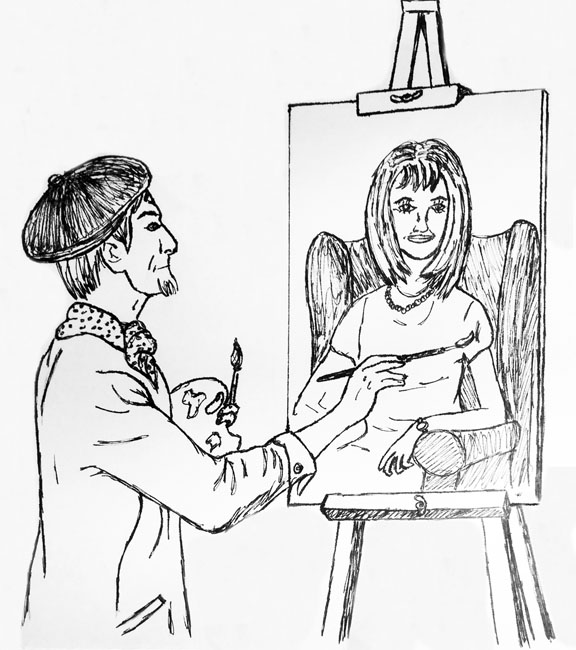
\includegraphics[trim=0 50 0 20,clip,width=0.28\columnwidth]{figures/exampleprompt.jpg}} &
\textbf{Response (L1)} \\
\cline{2-2}
& He is droning his wife pitcher. (Ar) \\
\cline{2-2}
& The artist is drawing a pretty women. (Ch) \\
\cline{2-2}
& The artist is painting a portrait of a lady. (En) \\
\cline{2-2}
& The painter is painting a woman's paint. (Sp) \\
\hline
\end{tabular}
\egroup
\end{center}
\caption{Example item from the pilot study showing responses from native speakers of Arabic (Ar), Chinese (Ch), English (En) and Spanish (Sp).}
\label{fig:example-picture}
\end{figure}
\end{small}
\vspace{-1em}
\pause
\begin{itemize}
\item 10 (transitive) PDT items $\times$ 53 participants $=$ 530 responses;
\pause
\begin{itemize}
\item 14 NSs (grad students), 39 NNSs (ESL students);
\end{itemize}
\pause
\item Annotation: \textit{Given the prompt, would the response be acceptable to most English speakers? Acceptable/unacceptable}
\begin{itemize}
\item 1 annotator (me)
\end{itemize}
\pause
\end{itemize}
\end{frame}

\begin{frame}
\frametitle{Pilot study: Processing}
\normalsize

First approach: \textbf{Rule-based} triple extraction and matching

\medskip
\pause
Dependency parser $\rightarrow$ lemmatizer $\rightarrow$ \textit{V(S,O)} extraction rules;

\pause
\medskip
Compare NNS \textit{V(S,O)} \& NS \textit{V(S,O)} list $\rightarrow$ covered / not covered;
\pause

\begin{itemize}
\pause
\item Dependency-based
\begin{itemize}
\pause
\item Captures aspects of form and meaning;
\pause
\item Subjects, objects, verbs clearly labeled;
\end{itemize}
\pause
\item V(S,O) extraction
\begin{itemize}
\pause
\item Decision tree based on dependency indexing \& labels, POS;
\pause
\item Custom for my transitive PDT, not generalizable, not robust;
\pause
\item $\approx$92\% accurate, $\approx$8\% extraction errors;
\end{itemize}
\pause
\item Overall accuracy: 58.9\%
\pause
\begin{itemize}
\pause
\item I.e., \textit{Acceptable} covered, \textit{unacceptable} not covered;
\end{itemize}
\end{itemize}
\end{frame}

\begin{frame}
\frametitle{Pilot study: Processing}

\normalsize
Second approach: \textbf{Semantic similarity} scoring

\medskip
\pause
Dependency parser $\rightarrow$ lemmatizer $\rightarrow$ term frequency-inverse document frequency (tf-idf; ``term'' $=$ lemmatized dependency);

\pause
\medskip
NNS response score $=$ cosine distance of NS and NNS tf-idf scores;
\pause

\begin{itemize}
\pause
\item tf-idf: Score dependencies according to importance; 
\pause
\item Vectorize \& Score
\begin{itemize}
\pause
\item Get \textit{sorted union set} of NS and NNS dependencies;
\pause
\item NNS vector: Replace deps with their \textbf{NNS} tf-idf scores;
\pause
\item NS vector: Replace deps with their \textbf{NS} tf-idf scores;
\pause
\item Response score $=$ \textit{cosine distance} for NNS \& NS vectors;
\end{itemize}
\pause
\item Rank by scores \& calculate Mean Average Precision (MAP);
\begin{itemize}
\pause
\item MAP \textit{acceptable} responses: $\approx$51\%
\end{itemize}
\pause
\item Process is more robust \& generalizable;
\pause
\item Dataset (especially NS models) and annotation are weak;
\end{itemize}
\end{frame}

\begin{frame}
\frametitle{System configuration}
\small

\vspace{-.5em}
\pause
All parameters or variables and their settings:

\vspace{-.7em}
\begin{table}
\begin{center}
\begin{tabular}{|l|l|l|l|l|}
\hline
\textbf{Trans\-i\-ti\-vi\-ty} & \textbf{Tar\-get\-ing} & \textbf{Fam\-il\-iar\-i\-ty} & \textbf{Prim\-a\-cy} & \textbf{Term Rep.} \\
\hline
\hline
\param{in\-trans\-i\-tive} & \param{tar\-get\-ed} & \param{familar} & \param{prim\-a\-ry} & \param{ldh} \\
\hline
\param{trans\-i\-tive} & \param{un\-tar\-get\-ed} & \param{crowd\-sourced} & \param{mix\-ed} & \param{xdh} \\
\hline
\param{di\-trans\-i\-tive} & & & & \param{xdx} \\
\hline
\end{tabular}
\label{tab:all-params}
\end{center}
\end{table}

\vspace{1.2em}
A \textbf{system configuration} combines one setting from each column.

\vspace{1.2em}
If particular settings correlate highly with item characteristics (intransitive / transitive / ditransitive; response complexity), I can optimize the system for new items.

\end{frame}


\begin{frame}
\frametitle{Sampling data: Response length}
\small
\begin{table}[htb!]
\begin{center}
\setlength{\tabcolsep}{.5em}
\begin{tabular}{|l||l|l|l||l|}
\hline
  & \multicolumn{2}{c|}{n=14} & n=50 & n=70\\
\hline
   & \param{Fam} & \param{Crowd} & \param{Crowd} 	& NNS			\\ \hline
\hline
\param{Intrans} & 5.5 	  		& 4.9 			& 4.9 		& 4.9 			\\ \hline
\param{Trans}   & 6.9          	& 6.3          	& 6.2       & 6.7    	    \\ \hline
\param{Ditrans} & 7.8          	& 7.2          	& 7.2       & 8.3    	    \\ \hline
\hline
\param{Target}  & 6.5 			& 5.4	 		& 5.4 		& 6.3			\\ \hline
\param{Untarg}  & 6.9        	& 6.8        	& 6.8    	& 6.9        	\\ \hline
\hline
\param{prim\-a\-ry} & N/A        	& 5.7 			& 5.8		& 6.6		 	\\ \hline
\param{mix\-ed}   & 6.7          	& 6.5          	& 6.4       & N/A	        \\ \hline
\hline
Total	& 6.7			& 6.1			& 6.1		& 6.6			\\ \hline
\end{tabular}
\caption{\label{tab:response-length}Comparing average response length (in words) for the samples used throughout this chapter as NS models and NNS test sets, in total and by parameter setting.}
\end{center}
\end{table}

\end{frame}

\begin{frame}
\frametitle{Annotation features}

\normalsize
\pause
%Feature requirements:
%\begin{itemize}
%\pause
%\item \textit{reliablity}: consistently annotated by multiple humans;
%\pause
%\item \textit{validity}: directly testing for the desired constructs;
%\end{itemize}
%\pause
First iteration: \textbf{accuracy (A)} \& \textbf{native-likeness (NL)}
\begin{itemize}
\pause
\item \textbf{2}: $+$A, $+$NL $>$ \textbf{1}: $+$A, $-$NL $>$ \textbf{0}: $-$A, $-$NL
\pause
\item Not operationalizable: e.g., response is accurate w.r.t. prompt but adds unverifiable details; is this still \textit{accurate}?
\item Not \textit{reliable}, not \textit{valid};
\end{itemize}
\pause
This was scrapped and I settled on the 5 binary features.

\end{frame}


\begin{frame}
\frametitle{Annotation features}

\normalsize
\pause
Inter-rater reliability for two annotators and 10\% of the dataset:
\pause

\textit{yes} annotations for Annotator 1 (note skewedness), expected chance agreement (\textit{Chance}), actual observed agreement (\textit{Observed}) and Cohen's kappa (\textit{Kappa})

\begin{table}[htb!]
\begin{center}
\begin{tabular}{|l|l||l|l||l|}
\hline
Set	& A1Yes & Chance & Observed & Kappa \\
\hline
\hline
Core Event & 0.733 & 0.601 & 0.923 & 0.808 \\
\hline
Answerhood & 0.834 & 0.721 & 0.982 & 0.936 \\
\hline
Grammaticality & 0.861 & 0.768 & 0.960 & 0.827 \\
\hline
Interpretability & 0.818 & 0.682 & 0.919 & 0.744 \\
\hline
Verifiability & 0.845 & 0.719 & 0.968 & 0.884 \\
\hline
%\pause \\
\hline
Intransitive & 0.863 & 0.758 & 0.978 & 0.910 \\
\hline
Transitive & 0.780 & 0.653 & 0.949 & 0.853 \\
\hline
Ditransitive & 0.812 & 0.678 & 0.924 & 0.764 \\ 
\hline
\end{tabular}
\end{center}
\end{table}
\end{frame}


\begin{frame}
\frametitle{Weighting features}
\begin{small}
\vspace{1ex}
Raters perform holistic preference test (blind to annotations)
\pause
\vspace{-2ex}
\begin{table}
%\scriptsize
\footnotesize
\begin{center}
\bgroup
\def\arraystretch{1.1}
\begin{tabular}{|=l|+c||+c|+c|+c|+c|+c|}
\hline
\textit{What is the boy doing?} & Pref? & Core & Ansr & Gram & Intrp & Verif \\
\hline
\hline
\rowstyle{\color{RoyalBlue}}He is eating food. & \textbf{yes} & \textbf{0} & \textbf{1} & \textbf{1} & \textbf{1} & \textbf{1} \\
\hline
\rowstyle{\color{Maroon}}He may get fat eating. & no & 0 & 0 & 1 & 1 & 0 \\
\hline
\pause \\
\hline
\only<2->{\rowstyle{\color{Maroon}}He is hungry. & no & 0 & 0 & 1 & 0 & 1} \\
\hline
\uncover<2->{\rowstyle{\color{RoyalBlue}}the boy is eating pizza & \textbf{yes} & \textbf{1} & \textbf{1} & \textbf{1} & \textbf{1} & \textbf{1}} \\
\hline
\pause \\
\hline
\only<3->{\rowstyle{\color{RoyalBlue}}{\scriptsize The child is about to eat pizza.} & \textbf{yes} & \textbf{1} & \textbf{0} & \textbf{1} & \textbf{1} & \textbf{1}} \\
\hline
\uncover<3->{\rowstyle{\color{Maroon}}he eating. & no & 0 & 1 & 0 & 1 & 1} \\
\hline
\pause \\
\hline
\only<4->{\rowstyle{\color{RoyalBlue}}Totals preferred responses & & 2 & 2 & 3 & 3 & 3} \\
\hline
\uncover<4->{\rowstyle{\color{Maroon}}Totals dispreferred responses & & 0 & 1 & 2 & 2 & 2 \\
\hline
\rowstyle{\color{RoyalBlue}}Net preferred (pref {\color{black}-} {\color{Maroon}dispref}) & & 2 & 1 & 1 & 1 & 1 \\
\hline
Feature weight &  & .333 & .167 & .167 & .167 & .167} \\
\hline \pause \\
%\multicolumn{7}{c}{} \\
\hline
\only<5->{}
\uncover<5->{$^*$Real feature weight &  & .365 & .093 & .055 & .224 & .263} \\
\hline
\end{tabular}
\egroup
\end{center}
\end{table}
\end{small}
\end{frame}


\end{document}